For \textbf{first} example, it given that there are total 4 nodes and 5 edges. Then next 5 lines represent 5 weighted edges.

Also in the string ``..x.", it is given that Node 3 is blocked initially, hence graph will look like this.
\begin{center}
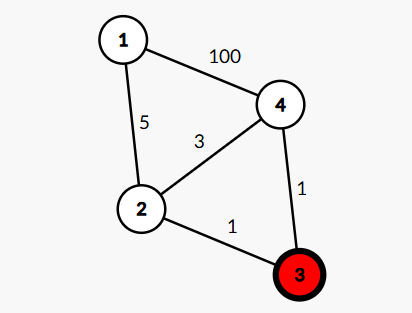
\includegraphics{q1-graph.png}
\end{center}
Orignally path 1, 2, 4 is taken which costs $ 5 + 3 = 8 $ while once Node 3 is toggled (and hence unblocked) path 1, 2, 3, 4 is taken which costs $ 5 + 1 + 1 = 7 $.

Similarly for the \textbf{second} example graph goes as follows after each toggle.
\begin{center}
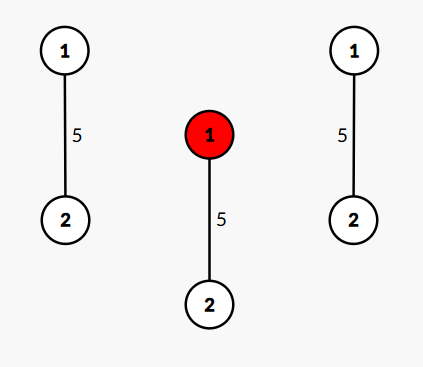
\includegraphics{q2-graph.png}
\end{center}
Initially 
\begin{itemize}
\item 1 to 2 is possible and cost is 5.
\item 1 to 1 is possible and cost is 0.
\item 2 to 2 is possible and cost is 0.
\end{itemize}
After blocking Node 1:
\begin{itemize}
\item 1 to 2 is not possible and hence print -1. (Since 1 is blocked)
\item 1 to 1 is not possible and hence print -1. (Since 1 is blocked)
\item 2 to 2 is possible and cost is 0.
\end{itemize}